\section{Segmentation of Myotubes with MyoSAM}
Alas, typical myotubes cannot be represented as star-convex polygons since oftentimes they have slight constrictions (cf. Fig.~\ref{figtubeblast}) or even bifurcations. In order to be able to segment those, it was necessary to turn to a foundation model. The Segment Anything Model \cite{kirillov2023segment} (\sam) lays claim to this title. It is a promptable image segmentaion model based on an encoder-decoder network that can be used for downstream segmentation problems. Much of \texttt{SAM} was inspired by advances made in natural language processing (NLP).
By visual inspection of its zeroshot performance, it becomes evident that it needs to be trained on suitable data. While it does a good job segmentating a lot of the structures, it also tends to oversegment noisy details or the cell nuclei. In addition to that, it runs into problems with the overlapping myotubes and does not find the second part of the tube in its entirety.
\begin{figure}
	\centering
	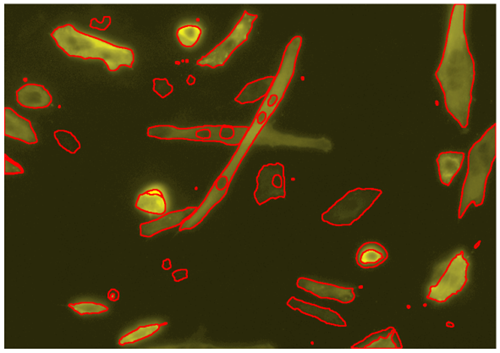
\includegraphics[width=\textwidth]{"images/sam_zeroshot.png"}
	\caption[\texttt{SAM} zeroshot]{Out-of-box application of the pretrained version of \texttt{SAM} to one patch of a myotube image.}
	\label{figzeroshot}
\end{figure}
\subsection{\texttt{SAM} Background}\label{SAMbg}
A high-level overview of \texttt{SAM} can be gained thorugh Fig.~\ref{figsamoverview}. The broad idea behind the model is simple: there needs to be a way to independently embed both prompt and image in order to jointly predict masks. The model therefore mainly consists of image encoder, prompt encoder, and a decoder network.
\begin{figure}
	\centering
	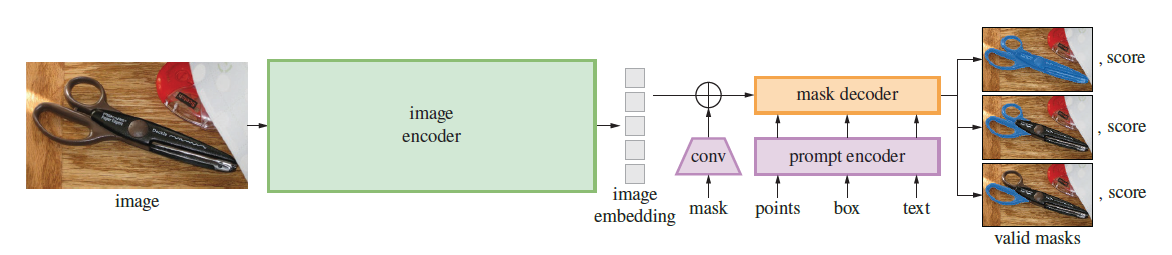
\includegraphics[width=\textwidth]{"images/sam_overview.png"}
	\caption[\texttt{SAM} Overview]{High-level overview of the two encoder networks interact to predict segmentation masks. Source: \cite{kirillov2023segment}.}
	\label{figsamoverview}
\end{figure}
A modified vision transformer \cite{dosovitskiy2020image} (ViT) is used as the image encoder. When applying ViTs the input image is divided into fixed-size patches. Each patch is embedded and treated as a token analogous to words in text tying in with the similarities to NLP. One dimensional positional encodings are added in order to retain spatial information. The image embeddings, along with positional encodings, are fed into a transformer encoder \cite{vaswani2017attention} consisting of attention blocks and feedforward neural networks, enabling the model to capture global dependencies between patches. Following the transformer encoder, the output is pooled to generate a fixed-size representation of the entire image, which is subsequently processed by fully connected layers for the final task. This approach offers benefits such as global context understanding, scalability to larger image sizes, and fewer inductive biases compared to traditional convolutional neural networks. Images are rescaled and padded to have a resoultuion of 1024 x 1024. The image embedding is of size 64x64 and convolved twice to get to 256 x 64 x 64.

While the image encoder is allowed to be computationally expensive since it only needs to be applied one time per image, the prompt encoder should be fast to guarantee the ability to set many prompt at once. \texttt{SAM} allows for two types of prompts: sparse (text, boxes, points) and dense (masks) ones. As only point prompts were used in this work, only those will be discussed in the following and will simply be referred to as prompts. In order to encode the prompts, two pieces of information are required: foreground/background and position knowledge. The positional encoding is either summed with an embedding for the foreground or one for background to form a 256 dimensional vectorial embedding.

Both types of embedding are then included into the decoder network. The decoder is depicted in Fig.~\ref{figdecoder} and its primary part consists of four steps. These four steps are performed twice to update both image and prompt embeddings. In addition to the prompt embeddings, an output token is introduced and the combination their combinatation is then referred to as tokens. This is the only stage where there is any sort of information exchange between prompt and image. In the first step, self-attention is applied on the tokens. Afterwards the tokens are used as queries to compute the cross-attention to the image embeddings\footnote{Note that image embeddings go hand in hand with their positional embedings, too.}. As a thrid step, a multi-layer-perceptron (MLP) updates the tokens. Eventually, the complement of the second step is performed: the cross attention of image to tokens. The learned image embeddings, which are now aware of the prompt information, are upsampled through transposed convolutions and, at the same time, are attented to once more by the tokens. A 3-layer MLP is used to transform these tokens to a dimension so as to match the upscaled image embeddings. A pointwise product between this MLP's output and the upscaled image embeddings results in the prediction of the mask. The aforementioned output token is used within a second head to predict values for the intersection over union (IoU) to the ground truth. In order to remove ambiguity due to a given prompt, several (three by default) masks are predicted and ranked by their IoU scores. During training only masks with the highest IoU are used for the calculation of the loss. 

It remains to discuss the trainings loop. Interactive segmentation is simulated during training by randomly selecting foreground point sampled uniformly from the ground truth mask $G = (g_{i})$ and selecting subsequent points from the error region (both false positive and false negative) between the previous (binary) mask prediction $M$  and the ground truth, with each new point classified as foreground or background based on what type of error region $E$ it was sampled from. A mask prediction is provided from the previous iteration as an additional prompt, using unthresholded mask logits $P = (p_{i})$ to maximize information transfer. When multiple masks are returned, the one with the highest predicted IoU is used for the next iteration. After eight iteratively sampled points diminished returns are observed. Two additional iterations are included without new external information to allow the model to refine its predictions. One such iteration is performed at the very end and one is introduced at a random spot. This results in a total of 11 iterations, balancing the use of external guidance with the model's own learning. This lightweight mask decoder allows for a relatively large number of iterations with minimal computational overhead compared to previous methods. The loss that is used is made up of three components: dice loss, focal loss \cite{liu2009otsu}, and IoU loss. The latter is just the penalization of the IoU prediction and is nothing but the mean squared error. The dice loss penalizes predictions by the percentage of misclassified pixels. The focal loss is a modification of the cross entropy loss with a modulation factor $\gamma$ to scale down the loss assigned to well-classified examples.  All in all, the loss takes the form
\begin{equation}\label{samloss}
	L_{\text{train}} = L_{\text{dice}} + 20L_{\text{focal}}+ L_{\text{IoU}} = \left(1 - \dfrac{2|M \cap G|}{|M| + |G|}\right) - 20\sum_{i}(1-p^t_i)^{\gamma}\log p^t_i + \|\text{IoU}_{\text{pred}} - \text{IoU}_{\text{gt}}\|_{L^2}^{2},
\end{equation}
where $|\cdot|$ denotes the number of pixels of an area and the logits are defined as
\begin{equation*}
	p_i^\text{t}=\begin{cases}p&\text{if}\quad g_i=1\\1-p&\text{if}\quad g_{i}=0,\end{cases},
\end{equation*}
and the summation runs over all pixels. $\gamma = 2$ was used during training.

\begin{figure}
	\centering
	\begin{subfigure}{0.45\textwidth}
		\centering
		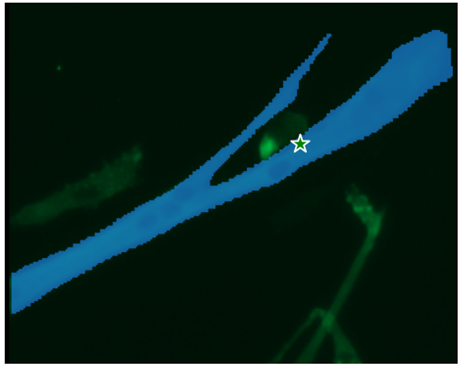
\includegraphics[width=\linewidth]{images/training1}
		\caption{First sampled point from the ground truth mask}
		\label{figtrain1}
	\end{subfigure}
	\hfill
	\begin{subfigure}{0.45\textwidth}
		\centering
		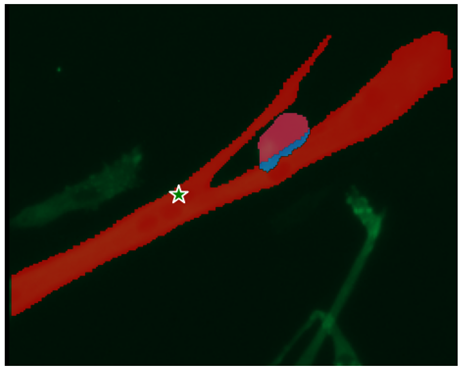
\includegraphics[width=\linewidth]{images/training2}
		\caption{Error region after the first prediction including new sampled point}
		\label{figtrain2}
	\end{subfigure}
	
	\medskip
	
	\begin{subfigure}{0.45\textwidth}
		\centering
		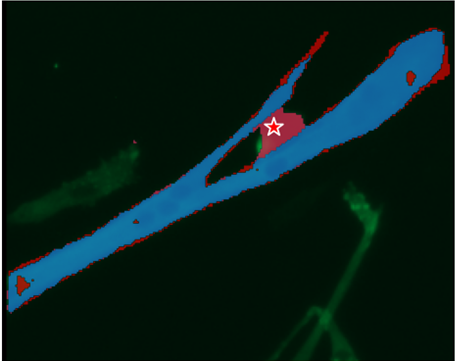
\includegraphics[width=\linewidth]{images/training3}
		\caption{New error region with another new point prompt}
		\label{figtrain3}
	\end{subfigure}
	\hfill
	\begin{subfigure}{0.45\textwidth}
		\centering
		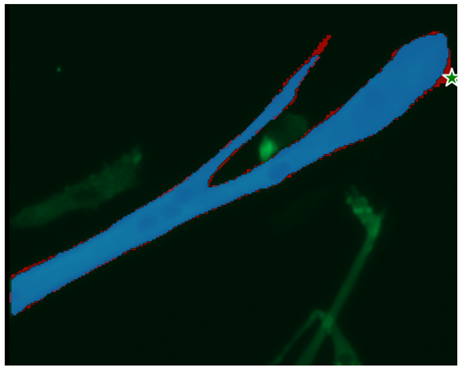
\includegraphics[width=\linewidth]{images/training4}
		\caption{Iteration beyond which resampling displays marginal return}
		\label{figtrain4}
	\end{subfigure}
	\caption[\texttt{SAM} trainings loop]{Exemplifying the main idea behind the \texttt{SAM} training loop}
	\label{figtrain}
\end{figure}

\begin{algorithm}
	\caption{SAM Training Algorithm}
	\begin{algorithmic}[1]
		\State Initialize ground truth mask $G$
		\State Initialize total number of iterations $n$
		\State Initialize logit mask $ P = \text{None}$
		\State Initialize threshold $t$
		\State Sample random integer $u\in \{k \in \mathbb{N}|k\leq n\}$
		\State Uniformly sample a foreground point $p$ from $G$
		\For{$i = 1$ to $n$}
			\State Predict new logit mask $P$ using point $p$ and logit mask $P$
			\If{i = u or i = n}
				\State \textbf{continue}
			\EndIf
			\State Update binarized mask $M_{\text{pred}} = P > t$ 
			\State Update error region $E = |G - M_{\text{pred}}|$
			\State Update point $p$ by sampling uniformly from error region $E$
			\If{$E(p)$ is false negative}
				\State $p$ is a foreground point
			\ElsIf{$E(p)$ is false positive}
				\State $p$ is a background point
			\EndIf
		\EndFor
	\end{algorithmic}
\end{algorithm}

\begin{figure}
	\centering
	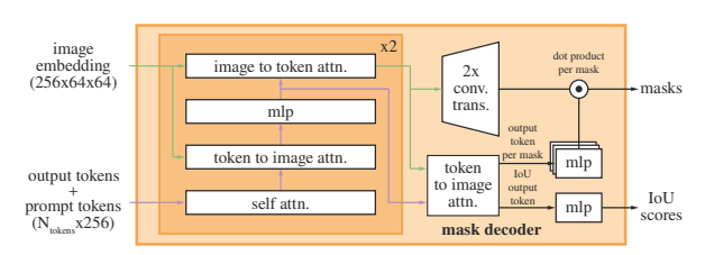
\includegraphics[width=\textwidth]{"images/maskdecoder.png"}
	\caption[\texttt{SAM} mask decoder]{Four attention steps in the mask decoder. Source: \cite{kirillov2023segment}.}
	\label{figdecoder}
\end{figure}

In order to not set all of the point prompts manually during segmentation, the SAMAutomaticMaskGenerator class was created. This allows to automatically set the number of points per side, the number of crops performed before setting these points, NMS thresholds, and many other scores in order to get many masks at once.